\section{\noah: Design Considerations}
\label{sec:design}
In this section,
we outline our design considerations
for a spreadsheet navigation interface.
%In our supplementary material,
%we additionally characterize
%the use-cases that such a navigation %interface
%is good for and not good for.
Our design considerations were
informed by prior work on
information visualization~\cite{shneiderman2003eyes,brehmer2013multi}, overview+detail interfaces~\cite{cockburn2009review}, multiple-coordinated views~\cite{wang2000guidelines},
and refined through our experiences
across multiple design iterations.

\para{DC1. Construct the overview in-situ}
An overview helps users get a high-level picture
of the data.
However, maintaining the overview in a separate
location from the data can \newsaj{lead to loss of context};
instead, having it co-located with the data
can help users make rapid glances to
explore information between a
bird's-eye view
and a close-up detail~\cite{grudin2001partitioning}.

\para{DC2. Ensure reduced
visual discontinuity while providing details on demand}
Users often need to access subsets of data,
and study their properties in detail, \eg via steering.
Navigating back and forth \saj{between different subsets of data}
can lead to increased visual discontinuity.
The interface should allow users to compute such details for
various data subsets on demand~\cite{shneiderman2003eyes}.
The interface should maintain visual continuity
as users navigate to a different subset,
recomputing the details for the new subset.

\para{DC3. Balance the screen space afforded to the overview}
As the overview
has limited screen-space available,
we need to consider the trade-off between visual discontinuity (\emph{DC2}) and clarity.
\saj{Displaying a fine-grained overview improves visual clarity while increasing visual discontinuity---users need to scroll through the overview to access distant
subsets of data.
Displaying a coarse-grained overview decreases visual discontinuity at cost of reduced visual clarity---the overview may span too many data subsets and appear visually cluttered}.
The interface should further allow users to control the screen-space allocated
to the overview.


\para{DC4. Enable coordination between the spreadsheet and overview}
Since users can view the overview
and the spreadsheet simultaneously,
interactions on both need to be linked~\cite{roberts2007state},
\ie an interaction on one should be reflected on
the other~\cite{wang2000guidelines}.
For example, as a user scrolls through
the spreadsheet, the user's current focus
should be highlighted on the overview.
However, not all interactions need to be interlinked,
\eg changing the font size of a spreadsheet cell
need not lead to a change in the overview.



\para{DC5. Facilitate customization of the overview}
As the overview is automatically generated,
it may not reflect domain-specific context
known only to the user~\cite{Raman99scalablespreadsheets}.
For example, an overview constructed on a grading
spreadsheet by binning nearby scores
may not match the letter grade ranges
that the instructors have in mind.
Allowing users to customize the overview is therefore essential.

\para{DC6. Display contextual and historical navigation information}
The interface should record navigation history,
allowing users to revisit previously visited locations~\cite{shneiderman2003eyes},
while also displaying their current navigation path for context.

\section{User Interface}
\label{sec:ui}
We now explain the design of \noah's components
and implementation details.

\subsection{In-situ Overview}

\noah constructs the overview in-situ ({\bf DC1})
next to the spreadsheet
on an attribute of the spreadsheet dataset
called the {\em navigation attribute},
selected by the user.
Any attribute type that can be ordered
can be a navigation attribute, \eg
text, numbers.
The overview is constructed at multiple granularities.
Each granularity is divided into non-overlapping
groups of data called {\em bins}.
As shown in Figure~\ref{fig:concept}d,
an overview of the Airbnb data
on the navigation attribute ``city''
has granularity levels.
The highest (coarsest) granularity level
consists of four bins.
Figure~\ref{fig:concept}a
depicts the first four bins,
the first of which is {\em Ashville-Boston}.
Each bin contains summary information
regarding the data subset/region
it spans, \eg starting row and
ending row number, and 
the total number of rows the region spans.
Each bin displays an overview
of the next (finer) granularity (if any)
with embedded bar charts.
For example, in Figure~\ref{fig:concept}d,
the topmost bin ({\em Ash-Bos}) spans three cities
({\em Ashville}, {\em Austin}, {\em Boston}), each of which is a bin
in the next (finer) granularity.
Correspondingly, Figure~\ref{fig:concept}(a)
shows three horizontal bar charts for the
first {\em Ash-Bos} bin,
one for each bin in the next granularity.
Since the third bin from the top
(\emph{LA}) spans only one city,
no bar chart is embedded.
Users can perform different
operations on the bins, \eg clicking to pan and
semantic zooming in/out~\cite{perlin1993pad}.
\noah supports other interactions,
\eg customization and aggregation.
We discuss these interactions
in the context of our design considerations in Section~\ref{sec:overview_operations}.

\stitle{Why a Multi-granularity Binned Overview?}
\saj{A standard overview approach
is to show a spatially partitioned
collection of thumbnails \saj{on the left of the detailed view},
similar to Microsoft PowerPoint or
Adobe Reader.
However, displaying too many thumbnails
results in increased scrolling
to access distant thumbnails,
increasing visual discontinuity.
On the other hand,
displaying too few thumbnails
reduces visual discontinuity,
but at the cost of visual
clarity---the thumbnails appear cluttered
and fail to represent the
underlying data clearly~\cite{cockburn2009review}.
To strike a balance between these two objectives
({\bf DC3}) we designed a multi-granularity overview
that abstracts the data at varying levels of detail.
Multi-granularity interfaces
provide an alternative to \newsaj{the spatially partitioned single-granularity representation of the data space, \eg in Powerpoint, by allowing users to control the scale at which the overview should be displayed~\cite{cockburn2009review}.}
Users can resize the overview to control the amount of spreadsheet data that remains visible.
\toappendix{Microsoft PowerPoint also uses a
similar technique to balance the screen
space between overview and detail.}
Users can also hide the overview if required.}

\newsaj{The data structure underlying the overview
is an equi-depth histogram constructed
on the values
in the navigation attribute column.
Equi-depth histograms are commonly
used for summarizing the statistical properties
of data, with applications such as
database query optimizers~\cite{chaudhuri1998random}.
The binned representation of the overview
using equi-depth histograms
enables faster navigation
by reducing visual discontinuity. 
The bins act as landmarks
in the overview, enabling 
users to skip irrelevant bins
and quickly navigate to the desired subset of data. We now discuss how the overview is constructed.}


\stitle{Overview Construction.}
\newsaj{The equi-depth histogram 
can be constructed on 
any data types
that can be ordered, \eg text, numbers, dates. For example, 
in the usage scenario explained in Section~\ref{sec:usage},
the journalist grouped the data into cities
for ease of navigation 
when exploring the larger cities
in the Airbnb dataset.}
Each bin in the equi-depth histogram
contains the same number of items,
where each item is a value.
For example,
when constructing the overview
on city,
each value in the city column
is assigned to a bin.
The bins are constructed top-down
(see Figure~\ref{fig:concept}d). \noah divides
each of the bins at level $k$ into new bins
to construct the next lower level $k+1$, again,
by applying the same concept of equi-depth histograms.
If each value of the navigation attribute
column was unique, \eg if it was a numerical ID,
then construction of the histogram would be easy:
each bin of the equi-depth histogram
would contain almost the same number of items,
where each item corresponds to one unique value of
the attribute.
Unfortunately, in practice, for many attributes,
the same value is often repeated.
For example,
there are multiple listings
per city.
Therefore,
an equi-depth histogram
on the
attribute city
will result in consecutive bins
sharing items of
the same unique city value,
resulting in undesirable overlap.
Instead,
we construct a best effort
equi-depth
histogram that is as close to an equi-depth
histogram as possible, while ensuring
that the ranges represented by each bin have no overlap.
\agp{Aditya: would be valuable to describe the algorithm to increase
technical depth.}
\saj{Saj: can we add a pseudocode in appendix and refer to that?}


\begin{figure}[t]
        \centering
        %\vspace{-10pt} %trim=left bottom right top
        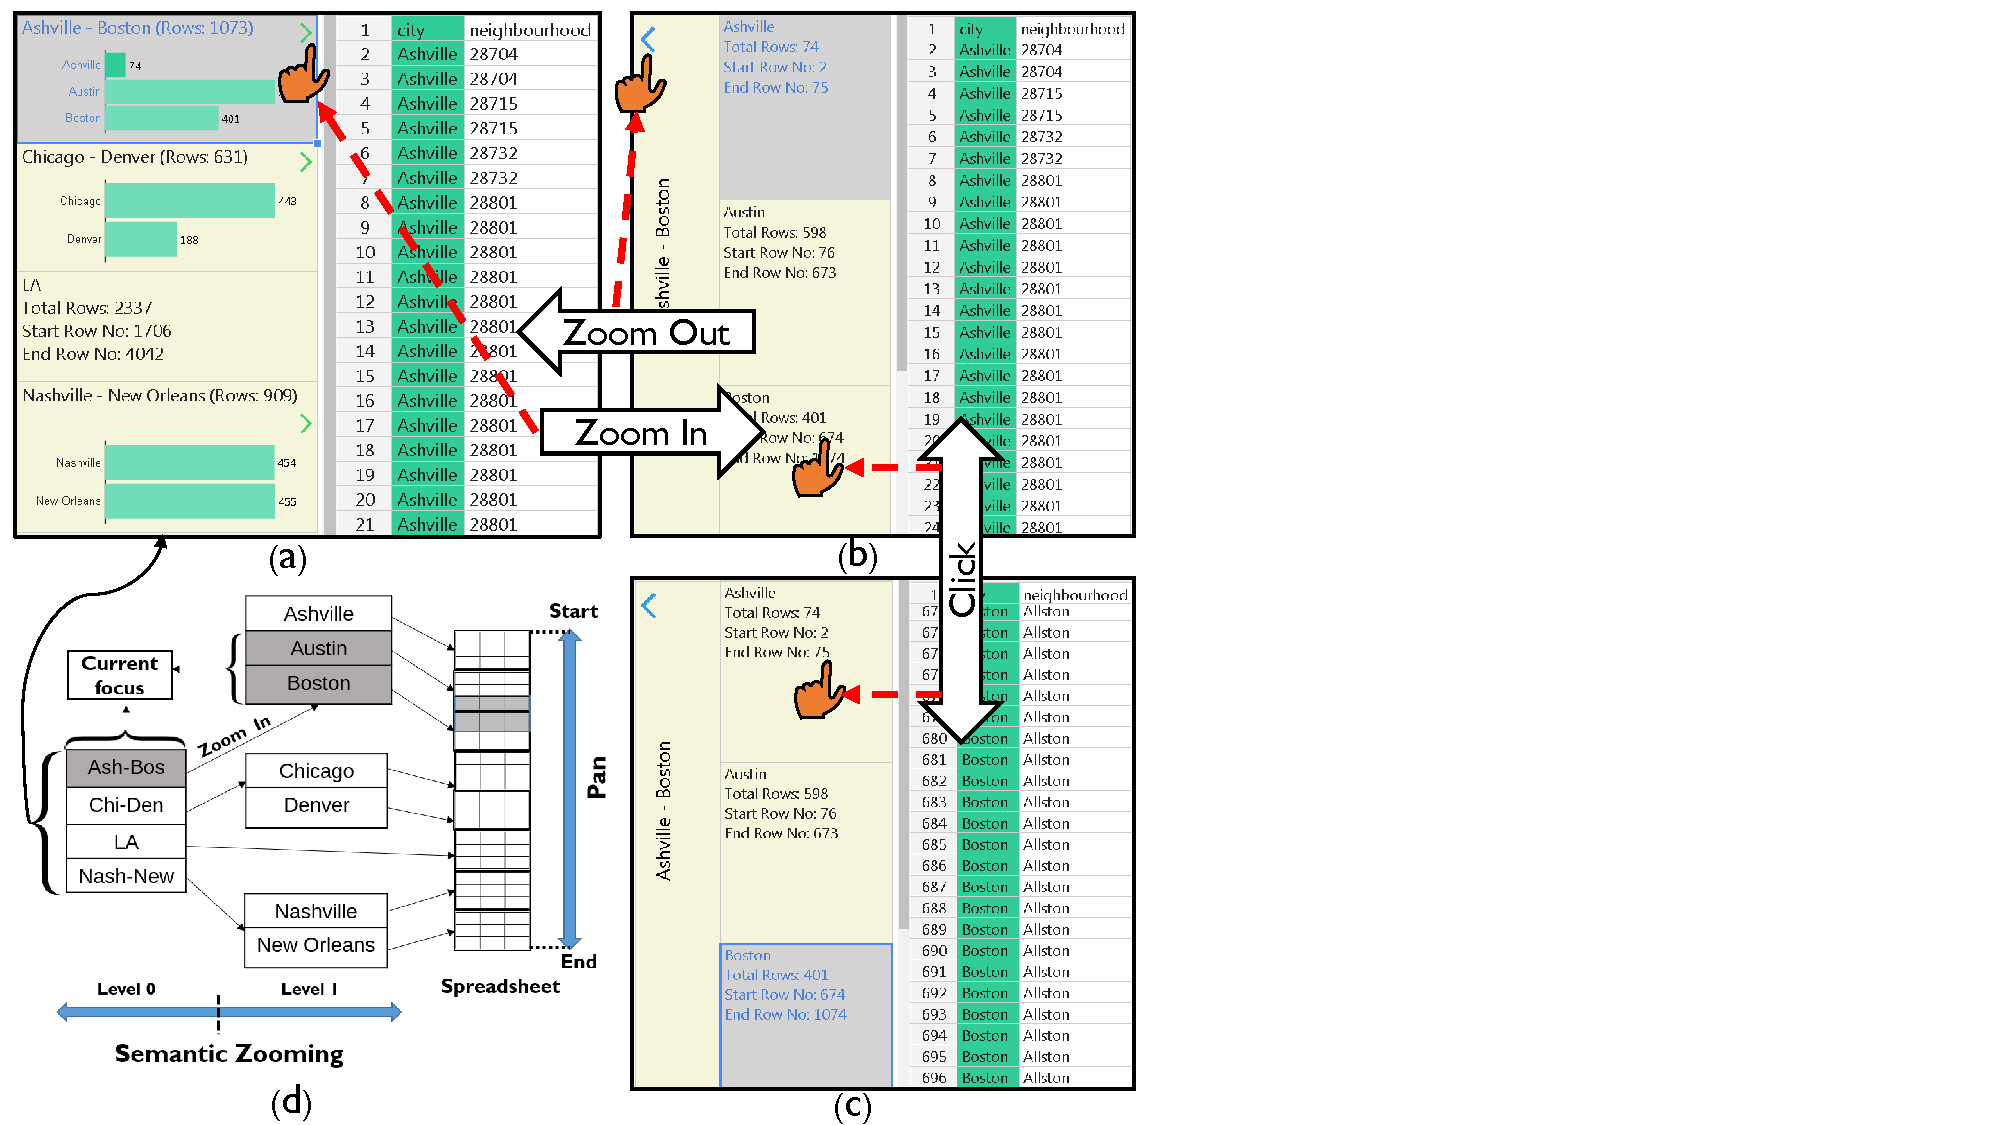
\includegraphics[width=0.45\textwidth,trim={0 0 400 0},clip]{images/navigationOp.pdf}
\vspace{-10pt}
   \caption{Navigational operations. (a) The overview at the highest level of granularity. (b) A zoomed in view of the \emph{Ashville-Boston} bin. (c) As the user clicks on the \emph{Boston} bin, the Boston listings are displayed on the sheet. The \emph{Boston} bin is highlighted in gray to indicate user’s current focus. (d) Conceptualizing the multi-granularity overview. }
\vspace{-18pt}
   \label{fig:concept}
 \end{figure}

\subsubsection{Operations and Interactions}
\label{sec:overview_operations}
We now discuss the operations and interactions that can be performed on the overview.

\stitle{Navigational Operation: Clicking.}
When a user clicks on a specific bin,
\noah displays the corresponding spreadsheet data;
users can use this to jump to a specific spreadsheet location
without having to scroll endlessly.
For example, in Figure~\ref{fig:concept}b,
as the user clicks on the \emph{Boston} bin,
the data corresponding to Boston is displayed
(Figure~\ref{fig:concept}c).
Note that the click operation is different from the traditional
spreadsheet \code{Filter} operation.
\code{Filter} hides spreadsheet data
that do not satisfy the filtering condition while
clicking brings the desired subset of data
in view without hiding the rest.
Users are free to navigate to other portions
through scrolling
even after clicking a bin, unlike filtering,
where users need to issue another \code{Filter}
to bring other data into view.


\stitle{Navigational Operation: Semantic Zooming.}  
Users can zoom into a specific bin
to view more fine-grained information or zoom out
to view more coarse-grained information,
via semantic zooming~\cite{perlin1993pad}.
For example, in Figure~\ref{fig:concept}a,
from the bin \emph{Ashville-Boston}
when the user zooms in to the next level,
\noah displays the bins \emph{Ashville}, \emph{Austin},
and \emph{Boston} (Figure~\ref{fig:concept}b).
If the user zooms out of the current granularity, again \noah displays the bins \emph{Ashville-Boston}, \emph{Chicago-Denver}, and others.
Users can only zoom into any bin that
contains multiple unique values.
For example, in Figure~\ref{fig:concept}d, at level 2,
each bin corresponds to one city.
Therefore, users can only click on those bins
to bring that data into view, and cannot zoom in further.
One issue with zooming interactions
is discoverability \saj{of the zoom operation}~\cite{cockburn2009review}.
We circumvent this (see Figure~\ref{fig:concept}c)
by providing the root of the bin under selection
for zoom out, and arrows for
clicking to zoom in (``\textcolor{blue}{$\rangle$}'') and out (``\textcolor{blue}{$\langle$}'').

\stitle{Customizing the Overview.}
As \noah constructs the overview automatically,
the overview binning or organization
may not capture domain-specific context
or user needs.
\noah enables users to customize\toappendix{ (\code{create} in Table~\ref{tab:scope})} this organization (\textbf{DC5}).
At any granularity, users can merge multiple consecutive bins
into a single bin, or split a bin into multiple bins.
\toappendix{The other operations include merging all the bins into one single bin and collapsing all the bins into singular bins, \ie one unique value per bin.}
Say the user wants to compare summary statistics
of Boston and Chicago.
In the current organization
these two cities are  
in two different bins (see Figure~\ref{fig:customize}a).
Using the bin customization feature,
the user can merge the two bins
\emph{Ashville-Boston} and \emph{Chicago-Denver} to create a new bin \emph{Ashville-Denver}.
Users can now zoom into this bin and
compare summary statistics of the cities in the same view.
The interactions for splitting a
bin depend on the data type.
If the navigation attribute is textual,
any bin can be split into as many bins as the
number of unique values that bin contains.
If the navigation attribute is numeric,
users can split the bin into any arbitrary number of bins.
Note that \noah does not allow users to rearrange the
order of the bins.\toappendix{ Users can only customize the boundary of the bins.} Since the overview represents a histogram, the bins are ordered---reshuffling the bins violates that order.

\begin{figure}[!htb]
        \centering
        \vspace{-8pt}
        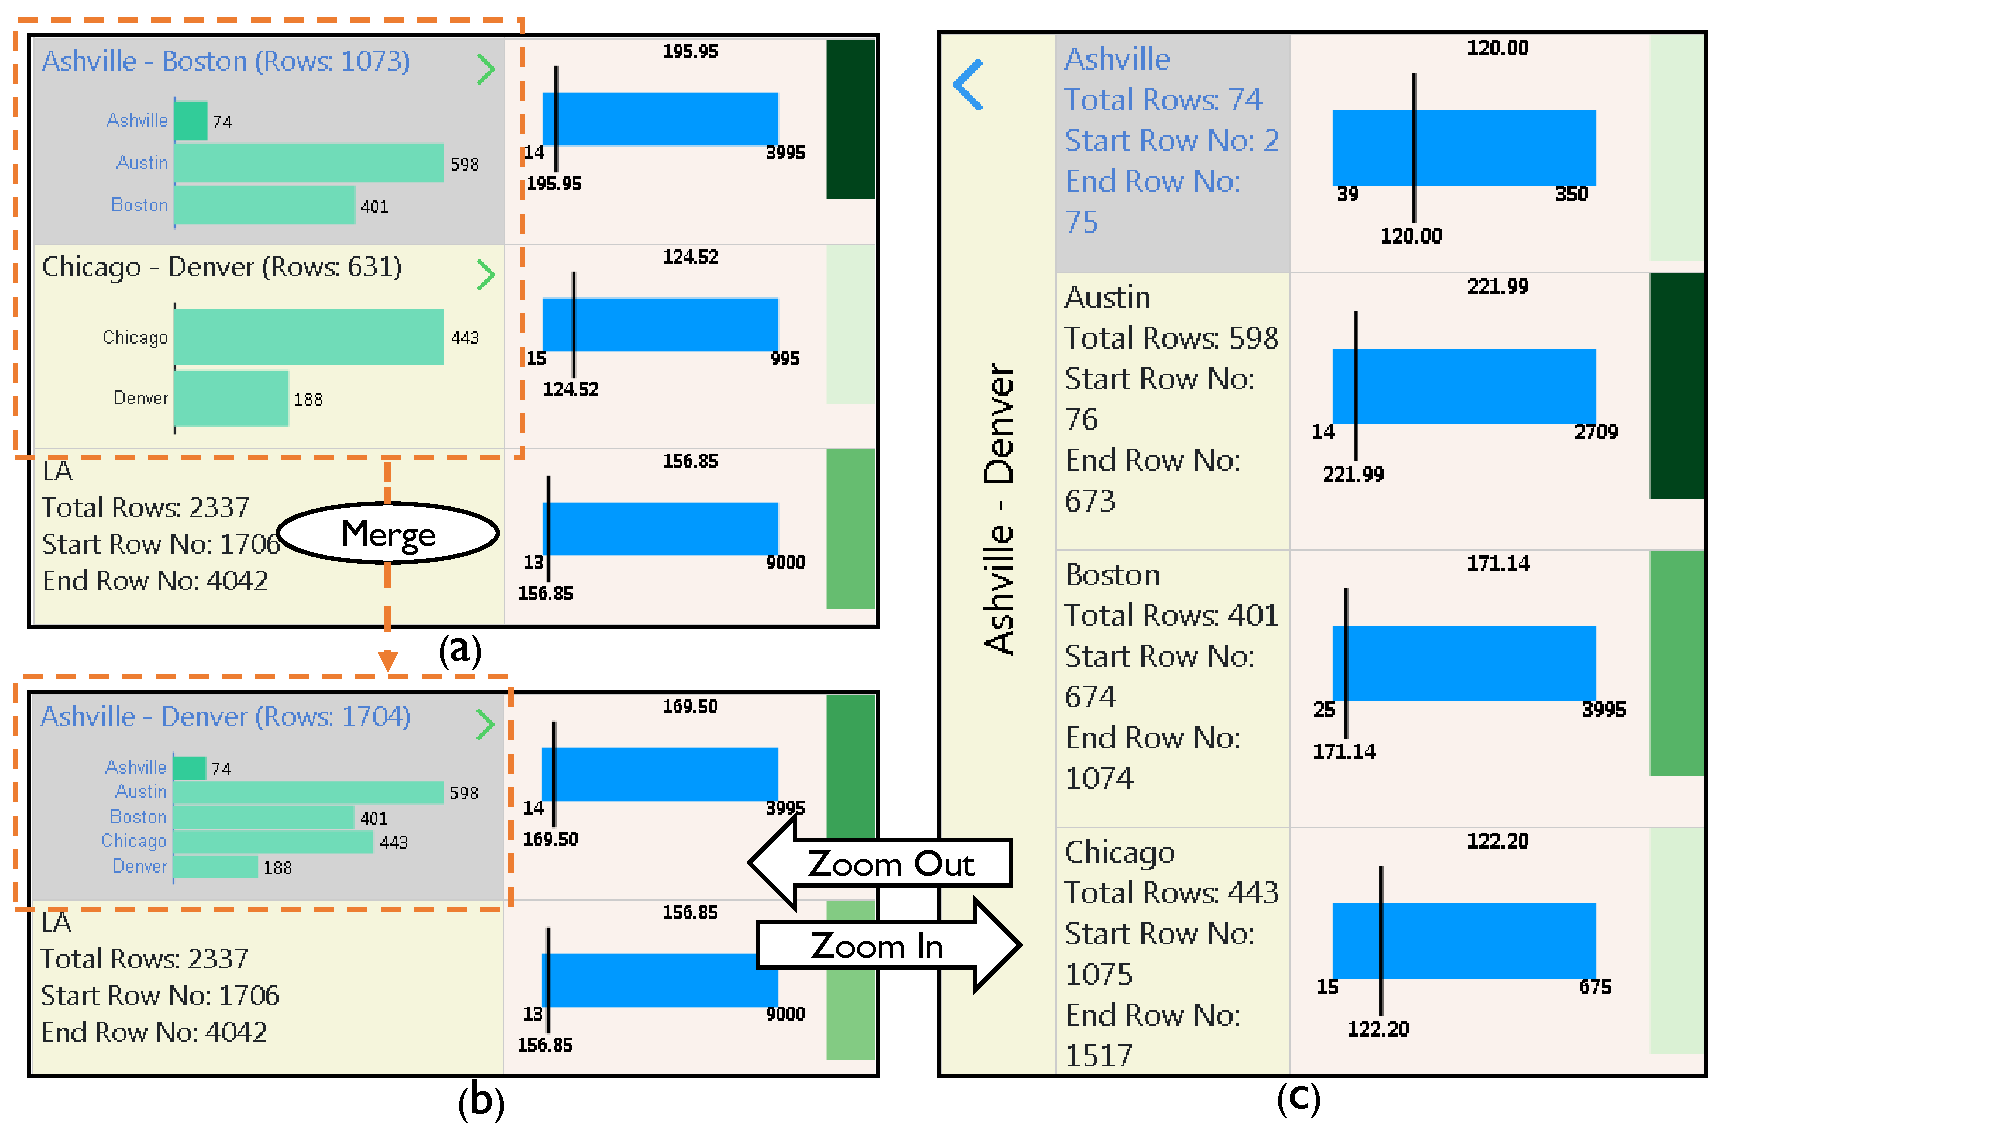
\includegraphics[width=0.45\textwidth,trim={0 0 130 0},clip]{images/customize.pdf}
\vspace{-10pt}
   \caption{(a) Chart view of the aggregate column. (b) A new bin is created by merging the top two bins. (c) Zooming into the newly created bin. }
\vspace{-10pt}
   \label{fig:customize}
 \end{figure}

\subsubsection{Coordination Between Overview and Spreadsheet}
\noah supports coordination
between the overview and the
corresponding spreadsheet data (\textbf{DC4}),
\ie interactions on the overview
may be reflected on the spreadsheet and vice-versa.
\newsaj{One example of this coordinations is,} indicating the navigation attribute on the spreadsheet
using color (see the lime green column in Figure~\ref{fig:ux}c)
as user constructs the overview. However, not all overview interactions are coupled
with the spreadsheet and vice versa.
The coupling depends on the user's current
focus---\emph{\saj{to ensure consistency between the overview and the spreadsheet,} any interaction on
either interface
that changes the current focus must be reflected
on the other interface}.
We now provide examples of both
coupled and decoupled interactions.

\stitle{Coupled interactions.}
Clicking a bin is an example of a coupled interaction
as the user actively changes the focus
to another bin on the overview.
To reflect the change, \noah populates
the corresponding spreadsheet data
on the screen.
As the user scrolls on the spreadsheet,
again the current focus changes
and the corresponding bin on the overview is highlighted.
For example, in Figure~\ref{fig:concept}c,
as the user clicks on the Boston bin,
the spreadsheet displays the Boston listings.
Conversely, as the user scrolls up,
both Austin and Boston listings appear in the current window of the spreadsheet.
Therefore, both the Austin and Boston overview
bins are highlighted
(see Figure~\ref{fig:concept}d).
%The zoom in operation, on the other hand,
%can be either coupled or decoupled based on the setting.
%Whenever a user zooms into a bin
%that is not the current focus,
%the spreadsheet is updated to show data
%for that bin.

\stitle{Decoupled interactions.}
When a user zooms into a bin
that is already in the user's current focus,
the spreadsheet view does not change.
For example, in Figure~\ref{fig:concept}a,
the user zooms into the \emph{Ashville-Boston} bin;
here, the spreadsheet view stays the same
(see Figure~\ref{fig:concept}b).
Similarly, the zoom out operation is decoupled.
When a user zooms out,
the overview displays
a coarser granularity view
of the user's current focus.
Since the focus stays the same,
there's no need to update the spreadsheet view.
Similarly, operations like panning on the overview without clicking,
and customizing the overview
do not change user's current focus and are therefore decoupled.
Online maps also adopt similar
decoupling of the overview and detail~\cite{cockburn2009review}.
However, their goal is to reduce network
and computational overload, whereas in our case,
the decoupling is based on the user's current focus.

\subsection{Aggregate Columns}
Users can issue spreadsheet formulae
on the overview
to compute aggregates for the data
in each bin\toappendix{ (\code{summarize} in Table~\ref{tab:scope})}.
The results
are displayed as an {\em aggregate column} (see Figure~\ref{fig:ux}b). Each entry in the aggregate column
corresponds to the adjacent bin
in the current granularity
of the overview.
For example, in Figure~\ref{fig:customize}c,
the aggregate column displays
four aggregate statistics,
one per bin.
Users can issue several formulae simultaneously,
each giving rise to a new aggregate column.
However, adding an aggregate column
takes up screen space, shrinking the spreadsheet view.
As a workaround, users can resize or
remove aggregate columns if required (\textbf{DC3}).
When the user issues a formula on the overview,
the spreadsheet column
corresponding to the aggregate column
is highlighted in grayish orange
(see Figure~\ref{fig:ux}c)---another example of coupled interaction.
For conditional formulae like \code{COUNTIF},
cells that satisfy the condition
are highlighted, \eg in Figure~\ref{fig:ux}c,
the cells with availability $\ge 60$ are colored in sky blue.
In this manner,
users can quickly determine which cells
are relevant to the aggregation operation\toappendix{ (\code{identify} in Table~\ref{tab:scope})}.

Creating an aggregate column on the overview mimics how users create pivot tables. Users
are not required to explicitly type formulae;
rather they simply select the formula from a drop-down menu,
and provide the necessary formula parameters to a form.
\newsaj{The aggregate column can employ any} statistical
and mathematical formulae that
operate over a range of data.
\newsaj{Therefore, creating an aggregate column
is equivalent to selecting subsets of data
on the sheet, \ie steering, and then executing a formula on this subset},
helping users avoid cumbersome steering operations.
We have classified the formulae supported
into five categories: a) summary (\eg min, max, average),
b) frequency (\eg mode, large, small), c) conditional (\eg countif, sumif), d) spread (\eg var,stdev), and e) others (\eg sum, count).

Users can view the results
either as raw values or as charts, and can toggle between the two.
Raw values are displayed
along with a colored bar, the \emph{value bar},
whose length is proportional to
the corresponding aggregate (see Figure~\ref{fig:ux}b). Users can use the lengths to visually compare across bins\toappendix{ (\code{compare} in Table~\ref{tab:scope})}.
The chart representation varies depending on the formula type.
All other categories except for the \emph{others} category
can be represented by charts.
Figure~\ref{fig:agg} shows the
chart representation for these categories
along with different visual cues
that highlight formula results
as well as other information. We discuss these representations 
in detail in the Appendix.
\toappendix{For example, for \emph{conditional} formulae
like \code{COUNTIF},
shading is used to de-emphasize data ranges
that do not satisfy the condition.
A similar shading technique is used for
the \emph{spread} category to highlight the standard deviation.
For the \emph{frequency} category,
coloring is used to identify the bin
with the result, \eg mode.
In the chart representation mode,
each entry of the aggregate column
contains one additional visual cue---a color bar
with shades of green on
the right of the chart (see Figure~\ref{fig:customize}).
The darker the color, the higher the value corresponding to that entry. Users can utilize the color intensity
to compare the results among different aggregate column entries.}


Finally, we note that the aggregate column
is kept in sync with the bins
as users zoom in and out,
eliminating repeated steering operations.
\noah does not maintain
any additional data structure for the aggregate column.
The histogram underlying the overview
records the result of the aggregate column entries
corresponding to the bins.
Next, we discuss how \noah maintains user's navigational context.

\begin{figure}[t]
%\vspace{-10pt}
{
\scriptsize
   \centering
\begin{tabular}{l|l}
   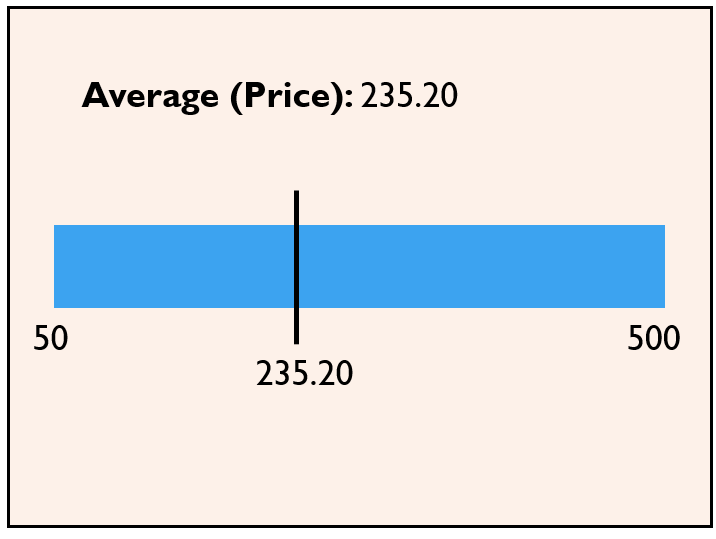
\includegraphics[width=0.20\textwidth]{images/summary.png} &
   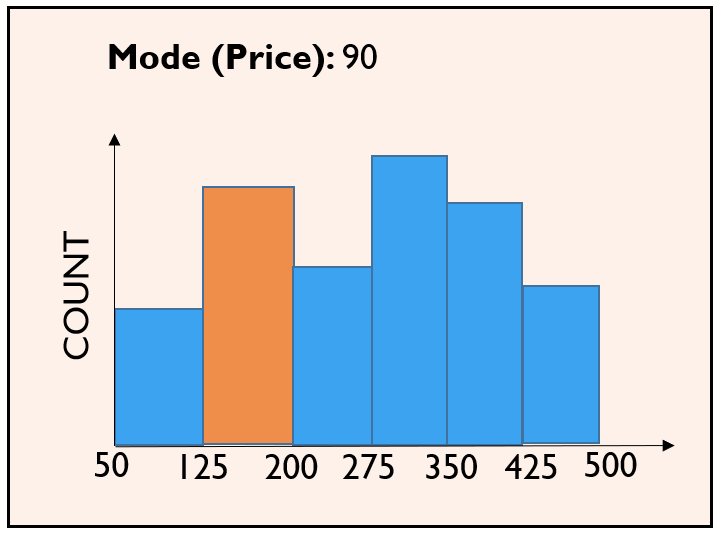
\includegraphics[width=0.20\textwidth]{images/frequency.png} \\
   \textbf{Chart Type:} Summary &  \textbf{Chart Type:} Frequency \\
 \textbf{Representation:} Horizontal bar &  \textbf{Representation:} Histogram \\
 \textbf{Visual Cue:} Vertical line (result) & 
 \textbf{Visual Cue:} Color (highlight) \\ \hline
    & \\
    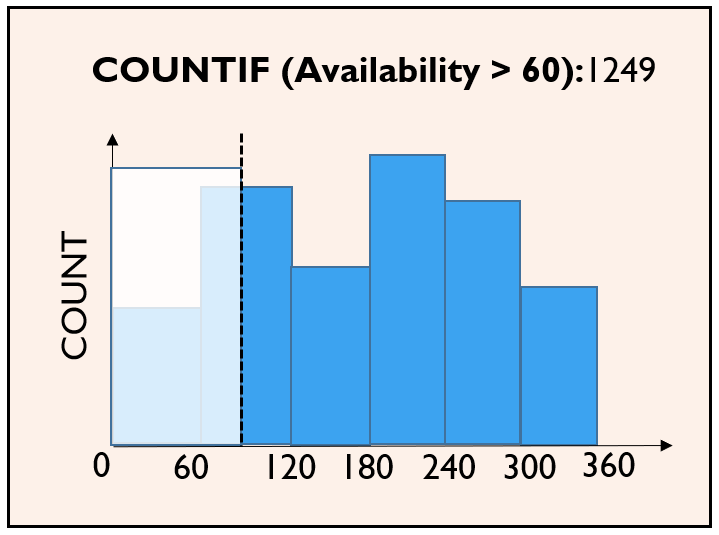
\includegraphics[width=0.20\textwidth]{images/conditional.png}  &
   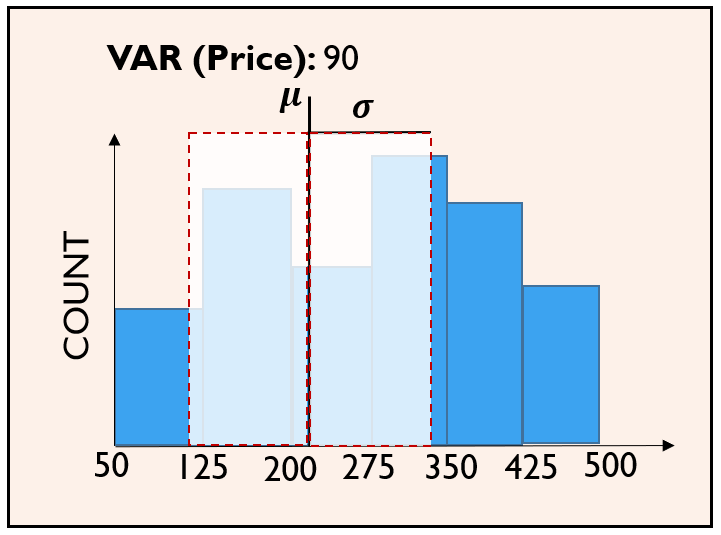
\includegraphics[width=0.20\textwidth]{images/spread.png} \\
      \textbf{Chart Type:} Conditional  &  \textbf{Chart Type:} Spread \\
 \textbf{Representation:} Histogram &  \textbf{Representation:} Histogram \\
 \textbf{Visual Cue:} Vertical line (result), & \textbf{Visual Cue:} Vertical line (mean),\\
Shade (de-emphasize) &  Shade (variance)
\vspace{-5pt}
\end{tabular}
}
\caption{Formula types and their chart representations.}
 \vspace{-15pt}
   \label{fig:agg}

\end{figure}
\subsection{Context Bar}
The context bar consists of two components:
a) a breadcrumb, and b) a navigation history.
The breadcrumb~\cite{breadcrumb} displays the current navigation path (see Figure~\ref{fig:ux}e), thus maintaining the users' navigation context (\textbf{DC6}). Each component of the breadcrumb corresponds to a bin in the user's current navigation path. Therefore, users can visit any bins within the current navigation path by clicking on an appropriate component of the breadcrumb, without having to zoom in or zoom out. \noah also maintains a list of recently visited bins (\textbf{DC6})
(see Figure~\ref{fig:ux}d). \toappendix{If aggregate columns are displayed along with the overview, contents of those columns are updated accordingly (\textbf{DC2}), as users revisit a bin.}

\subsection{Implementation}
We have integrated \noah with {\scshape DataSpread}~\cite{datamodels}, a web-based spreadsheet. The {\scshape DataSpread} back-end maintains the histogram data structure and  supports the aggregate column computation via its built-in formula engine.\toappendix{ To enable seamless integration of the overview with the spreadsheet data, we leverage the hierarchical positional indexes used by {\scshape DataSpread} to access
the spreadsheet data. The index is essentially an order statistics tree~\cite{datamodels} built on the position (\eg row number) of the spreadsheet data. For any given navigation attribute, a new positional index is constructed first. \noah then leverages the positional mapping to access the underlying data corresponding to the navigation attribute and constructs the histogram depicting the overview. Therefore, \noah can be integrated to any spreadsheet and requires only access to the positional mapping structure of that spreadsheet.} The \noah front-end is built with HTML/CSS/JS technologies along with the D3 framework~\cite{d3} for generating charts.






